%---------change this every homework
\def\yourid{njb2b}
\def\collabs{Dr. Seuss, Batman}
\def\sources{
    \textit{The Restaurant at the end of the universe} Adams,
    \url{https://simple.wikipedia.org/wiki/Al-Khwarizmi}
    }
% -----------------------------------------------------
\def\duedate{I have no idea when}
\def\duelocation{via Collab}
\def\hnumber{99}
\def\prof{Nate Brunelle}
\def\course{{cs3102 - Theory of Computation - Fall 2099}}%------
%-------------------------------------
%-------------------------------------

\documentclass[10pt]{article}
\usepackage[colorlinks,urlcolor=blue]{hyperref}
\usepackage[osf]{mathpazo}
\usepackage{amsmath,amsfonts,graphicx}
\usepackage{latexsym}
\usepackage[top=1in,bottom=1.4in,left=1.5in,right=1.5in,centering]{geometry}
\usepackage{color}
\definecolor{mdb}{rgb}{0.3,0.02,0.02} 
\definecolor{cit}{rgb}{0.05,0.2,0.45} 
\pagestyle{myheadings}
\markboth{\yourid}{\yourid}
\usepackage{clrscode}
\usepackage{url}
\usepackage{minted}
\usemintedstyle{bw}
\usepackage{enumitem}
\usepackage{ulem}
\usepackage{titling}
\setlength{\droptitle}{-5em}   % This is your set screw

\newenvironment{proof}{\par\noindent{\it Proof.}\hspace*{1em}}{$\Box$\bigskip}
\newcommand{\handout}{
   \renewcommand{\thepage}{H\hnumber-\arabic{page}}
   \noindent
   \begin{center}
      \vbox{
    \hbox to \columnwidth {\sc{\course} --- \prof \hfill}
    \vspace{-2mm}
    \hbox to \columnwidth {\sc due \MakeLowercase{\duedate} \duelocation\hfill {\Huge\color{mdb}H\hnumber.\yourid}}
      }
   \end{center}
   \vspace*{2mm}
}
\newcommand{\solution}[1]{\medskip\noindent\textbf{Solution:}#1}
\newcommand{\bit}[1]{\{0,1\}^{ #1 }}
%\dontprintsemicolon
%\linesnumbered
\newtheorem{problem}{\sc\color{cit}problem}
\newtheorem{practice}{\sc\color{cit}practice}
\newtheorem{lemma}{Lemma}
\newtheorem{definition}{Definition}


\begin{document}
\thispagestyle{empty}
\handout
\title{Assignment: Turing Machines}
\date{\vspace{-6em}}


\paragraph{Collaboration Policy} You are encouraged to collaborate with up to 3 other students, but all work submitted must be your own independently written solution. List the names of all of your collaborators. Do not seek published solutions for any assignments. If you use any published resources when completing this assignment, be sure to cite them. Do not submit a solution that you are unable to explain orally to a member of the course staff.

\paragraph{Objectives:}
\begin{enumerate}[nosep]
    \item Program a turing machine
    \item See the similarity between automata and real-world computer architectures
    \item Implement a parser for a turing machine's instruction set
    \item Implement a simulator for a turing machine's instruction set on an input tape
\end{enumerate}

\paragraph{Background} A turing machine is a finite state automata that can read from and write to an infinitely long input tape. It has a read head that can be moved along the tape, and can transition based symbols it reads from a cell. Based on this description, we have created an instruction set that directly maps to a turing machine's operations.\par
A \texttt{move <offset>} instruction shifts the read head on the input tape by the declared integer offset. For example, \texttt{move -2} shifts the read head to the left by two cells.\par
A \texttt{var <name>} instruction declares a variable with an associated name. A variable can store any printable ASCII character, either based on its integer value or character literal. The \texttt{read <name>} instruction stores the value held the tape's current cell into the variable with the associated name. To set a value on the tape, use the \texttt{write <operand>} instruction, which stores either an integer, character literal, or variable's value into the current cell. For example, after executing
\begin{verbatim}
    var x
    write 'a'
    read x
\end{verbatim}
both the current cell and the variable x hold the character 'a':\par
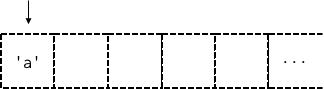
\includegraphics[scale=.5]{tm1}\\
But after executing the following,\par
\begin{verbatim}
    move 1
    write x
\end{verbatim}
the tape would then hold\par
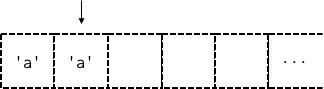
\includegraphics[scale=.5]{tm2}\\
It is possible to jump to any labeled line in the program. Simply declare a line to be a label with a \texttt{<name>:}, and use the \texttt{jump <name>} instruction to reposition the program counter to that line. For instance, after executing the following\par
\begin{verbatim}
    write 'c'
    jump end
    write 'a'
    end:
\end{verbatim}
the tape would hold\par
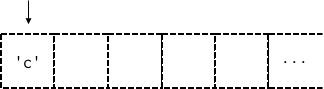
\includegraphics[scale=.5]{tm3}\\
The machine implements conditional branching with the \texttt{skipif <condition>} instruction. This instruction skips over the next line if the given condition holds true. The condition is a boolean expression that compares the equality of two operands. For example, if the tape initially contains\par
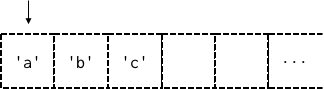
\includegraphics[scale=.5]{tm4}\\
and the following program is executed,\par
\begin{verbatim}
    var x
    read x
    skipif x == 'a'
    jump L
    write 'c'
    L:
\end{verbatim}
the jump instruction is skipped over, because the value of x is 'a'. The resulting tape contains\par
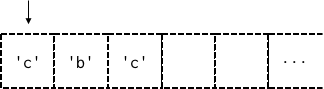
\includegraphics[scale=.5]{tm5}\\
A comment can be included on its own preceded with two forward slashes \texttt{//}. It is ignored during simulation.\par
The formal grammar for this instruction is given below. Note that it is context-free.\par
\begin{verbatim}
    SourceFile = InstructionList .
    InstructionList = { Instruction "\n" } [ Instruction ] .
    Instruction =
       Label ":" |
       "var" Identifier |
       "skipif" BooleanExpr |
       "move" Integer |
       "jump" Label |
       "read" Identifier |
       "write" Operand |
       Comment |
       ε .
    Label = Identifier .
    Identifier = letter { letter | digit } .
    letter = "a" … "z" | "A" … "Z" .
    digit = "0" … "9" .
    BooleanExpr = Operand ( "==" | "!=" ) Operand .
    Operand = Identifier | Integer | "'" character "'" .
    Integer = [ "+" | "-" ] digit { digit } .
    Comment = "//" text .
\end{verbatim}

\paragraph{Part 1 (40 points)} For this part, you must implement the following programs using the instruction set above. Test your programs by using the online simulator located at \href{https://www.tmsim.akhil.cc}{tmsim.akhil.cc}. Write each program in a file named \texttt{<program-name>.tm} for your submission.
\begin{enumerate}
    \item \texttt{increment.tm}: Write a program that takes as input a binary number in reverse, and increments it by one. For instance, the decimal number \texttt{6} would correspond to the input string \texttt{011}, and the incremented result would be \texttt{111}. Example test cases:\\
    {\renewcommand{\arraystretch}{1.2}
    \begin{tabular}{|r|r|}
     \hline
     Input & Output \\ [0.5ex] 
     \hline
     0 & 1 \\ 
     \hline
     01 & 11 \\
     \hline
     1 & 01 \\
     \hline
     11 & 001 \\
     \hline
     101 & 111 \\ [1ex] 
     \hline
    \end{tabular}
    }
    \item \texttt{palindrome.tm}: Write a program that is a decider for palindromes. That is, for $\sum = \{\texttt{'a'}, \texttt{'b'}, \ldots, \texttt{'z'}\}$, $L = \{w \in \sum^* \mid w$ is a palindrome$\}$. The result should be a tape only containing a \texttt{1} in the first cell if the decider accepts, and \texttt{0} in the first cell if the decider rejects. Example test cases:\\
    {\renewcommand{\arraystretch}{1.2}
    \begin{tabular}{|r|r|}
     \hline
     Input & Output \\ [0.5ex] 
     \hline
      & 1 \\ 
     \hline
     a & 1 \\
     \hline
     aa & 1 \\
     \hline
     ab & 0 \\
     \hline
     anna & 1 \\
     \hline
     madam & 1 \\
     \hline
     garage & 0 \\ [1ex] 
     \hline
    \end{tabular}
    }\\\\
    \textbf{Note: The program listed must match the file name! This is used for automated grading purposes!}
\end{enumerate}

\paragraph{Part 2 (30 points)}  In this part, you will implement a parser that takes in a program written in the instruction set above as a string, and returns a \texttt{List<Instruction>}. The required class declarations are located in \textbf{Parser.java}. The \texttt{Instruction} class is already provided for you in \textbf{Instruction.java}. You are not required to handle comments or empty lines. Additionally, you can assume that all of the tokens on a line are delimited by a single space. Run \textbf{TestParser.java} to run tests against the parser. Only valid programs will be tested against the parser.

\paragraph{Part 3 (30 points)} Here, you will implement a simulator that takes in a \texttt{List<Instruction>} and input tape, and returns the tape after executing the above instruction set. You are not required to handle invalid programs as all test programs are valid and halt. Run \textbf{TestSimulator.java} to run tests against the simulator.\par
\textit{Implementation notes}: Empty cells can be treated as whitespace characters. If a \texttt{read} or \texttt{write} instruction attempts to execute on input array of zero-length, grow the array to contain a whitespace character. Additionally, if a \texttt{move} instruction attempts to move past the end of the input array, grow the array to the appropriate size and initialize the remaining characters as whitespace.\par

\paragraph{Submission} When you are ready for submission, run \textbf{Submit.java} in the working directory containing all of your source files. This will produce a zip file that you should upload to collab.

%\paragraph{Collaborators} \collabs

%\paragraph{Sources} \sources

%----Begin your modifications here


%\begin{wrapfigure}{r}{3in}
%\epsfig{figure=water-slide-ink,width=3in}
%\vspace{-30pt}
%\end{wrapfigure}

\end{document}
